\chapter{Vers les bases de données graphe}
\label{ch:graph-db}
Avec le développement rapide et continu de l'Internet et le cloud
computing, divers types d'applications ont émergés, ce qui augmente
l'mportance accrue de la technologie de base de données, notamment
dans les aspects suivants \cite{han2011survey}:

\begin{itemize}
\item Haute concurrente de lecture et d'écriture avec une faible
  latence.
\item Stockage et la gestion d'une grande masse de données \emph{(Big
    Data)}.
\item Haute scalabilité (évolutivité) et disponibilité.
\end{itemize}

Bien que les bases de données relationnelles ont occupé une grande
position dans le domaine de stockage de données, le modèle relationnel
commençait à montrer ses limites en faisant face au-dessus exigences
\cite{han2011survey}:

\begin{itemize}
\item Lente lecture et l'écriture.
\item Capacité limitée.
\item Difficulté d'expansion et scalabilité.
\end{itemize}

Afin de faire face aux limitations ci-dessus, une variété de nouveaux
types de bases de données ont été apparus qui s'affranchissent du
modèle relationnel pour miser sur le partitionnement horizontal et le
relâchement des contraintes d'intégrité, ce modèle émergent est appelé
le modèle \acrshort{nosql}.

Dans ce chapitre, nous exposons les différentes approches et
plateformes du stockage \textsc{NoSQL} les plus connues dans
l'industrie tout en mettant l'accent sur les bases de données graphes
(et \emph{Neo4j} particulièrement). Nous commençons d'abord par
présenter les quatre catégories majeurs des systèmes
\textsc{NoSQL}. Ensuite, nous focalisons sur les \acrshort{SGBD}
orientés graphes, leurs différents modèles et implémentations ainsi
que les langages de requêtes les plus adoptés pour les interroger.

\section{L'environnement NoSQL}
\label{sec:nosql}
% TODO: make a real definition
\acrshort{nosql} désigne une catégorie de systèmes de gestion de base
de données (\acrshort{SGBD}) qui n'est plus fondée sur l'architecture
classique des bases relationnelles. L'unité logique n'y est plus la
table, et les données ne sont en général pas manipulées avec
\textsc{SQL}. À l'origine, servant à manipuler des bases de données
géantes pour des sites web de très grande audience tels que Google
Amazon, Facebook et eBay. D'aprés Martin fowler \textit{et al.}
\cite{sadalage2012nosql}, Les caractéristiques communes des bases de
données \acrshort{nosql} sont:

\begin{itemize}
\item Ne sont pas fondées sur de le modèle relationnel classique.
\item Optimisées pour les environments distribués.
\item Généralement sous des licences \emph{Open Source}.
\item Construites pour les applications Web modernes avec une grande
  masse de données.
\item \emph{Schemaless} (il n'existe plus d'intégrité référentielle ou
  schéma prédéfini).
\end{itemize}

  \subsection{Catégories des bases de données NoSQL}
  \label{sec:cat-nosql}
  Il existe dans la mouvance \acrshort{nosql} une diversité importante
  d'approches. que nous classons en quatre grandes catégories : dépots
  clés/valeurs, bases orientées documents, orientées colonnes, et
  bases orientées graphes.

  \begin{itemize}
  \item [Dépots clés/valeurs]: Le principe des bases
    \textit{clé/valeur} est de stocker les données sous une forme
    simple: une \emph{clé } (chaîne de caractères) associé à une
    \emph{valeur} d'une forme libre (chaîne de caractère, nombre ou
    bien un objet sérialisé), cette clé est utilisée pout toutes les
    opérations à effectuer sur les données telles que l'insertion, la
    mise à jour et la supression. Bien que la structure est plus
    simple, la vitesse d'interrogation est extrêmement supérieur à la
    base de données relationnelles favorisant la scalabilité
    (\emph{scalability}) plus que la cohérence, on les retrouve très
    souvent comme système de stockage de cache ou de sessions
    distribuées, notamment là où l'intégrité relationnelle des données
    est non significative. Les solutions les plus connues, telle que
    \emph{Redis}, \emph{Riak} et \emph{Voldemort} sont principalement
    influencés par le project \emph{Dynamo} d'Amazon
    \cite{decandia2007dynamo}.
    \newpage

  \item [Orientées documents]: Cette famille de base de données est
    une évolution de la base de données \textit{clé/valeur} destinée
    aux applications qui gèrent des documents (généralement du format
    \textsc{JSON} ou \textsc{XML}) où chaque clé n'est plus associée à
    une valeur sous forme de bloc binaire mais à un document dont la
    structure reste libre (\textit{scheme-less}). L'avantage est de
    pouvoir récupérer, via une seule clé, un ensemble d’informations
    structurées de manière hiérarchique. ansi que le stockage de
    volumes très importants de données pour lesquelles la modélisation
    relationnelle aurait entraînée une limitation des possibilités de
    partitionnement et de réplication. les deux implémentations les
    plus populaires dans cette catégorie sont \emph{CouchDB} d'Apache
    et \emph{MongoDB}.

  \item [Orientées colonnes]: Une base de données orientée colonnes
    est une base de données qui stocke les données par colonne et non
    par ligne. L'orientation colonne permet d'ajouter des colonnes
    plus facilement aux tables (les lignes n'ont pas besoin d'être
    redimensionnées). Elle permet de plus une compression par colonne,
    efficace lorsque les données de la colonne se ressemblent. Comme
    solutions, on retrouve principalement \emph{HBase},
    \emph{HyperTable} (implémentations Open Source du modèle
    \emph{BigTable} \cite{chang2008bigtable} publié par Google) ainsi
    que \emph{Cassandra} (projet Apache qui respecte l'architecture
    distribuée de \emph{Dynamo} \cite{decandia2007dynamo} d'Amazon et
    le modèle BigTable de Google).

  \item [Orientées graphes]: Ce paradigme est le moins connu de ceux
    de la mouvance \acrshort{nosql}. Ce modèle s'appuie principalement
    sur deux concepts: d'une part l'utilisation d'un moteur de
    stockage pour les objets (qui se présentent sous la forme d'une
    base documentaire, chaque entité de cette base étant nommée
    \emph{nœud}). D'autre part, à ce modèle, vient s'ajouter un
    mécanisme permettant de décrire les relations entre les objets
    (\emph{arcs}). Principalement, ces bases de données sont nettement
    plus efficaces que leur pendant relationnel pour traiter les
    problématiques liées aux réseaux.  En effet, lorsqu'on utilise le
    modèle relationnel, cela nécessite un grand nombre d'opérations
    complexes (souvent, des jointures trop lentes) pour obtenir des
    résultats. Dans cette catégorie on peut citer \emph{Neo4j},
    \emph{OrientDB}, \emph{Titan} et \emph{AllegroGraph} comme les
    implémentations les plus répondus de ce modèle.
  \end{itemize}

  \subsection{Le théorème de CAP }
  \label{sec:cap}

  \acrshort{cap} \cite{brewer2000towards} est l'acronyme de
  \textit{``\textbf{C}onsistency, \textbf{A}vailability and
    \textbf{P}artition Tolerance''}, ou \textit{``Cohérence,
    Disponibilité et Résistance au partitionnement''}. Ce théorème
  explique qu'il est impossible qu'un système distribué satisfasse
  simultanément aux trois contraintes suivantes:

  \begin{itemize}
  \item [Cohérence]: tous les nœuds du système voient exactement les
    mêmes données au même moment.

  \item [Disponibilité]: la perte de nœuds n'empêche pas les survivants
    de continuer à fonctionner correctement.

  \item [Résistance au partitionnement]: aucune panne moins importante
    qu'une coupure totale du réseau ne doit empêcher le système de
    répondre correctement (ou encore : en cas de partitionnement ,
    chacune des partitions doit pouvoir fonctionner de manière
    autonome).
  \end{itemize}

  \begin{figure}[h]
    \centering
    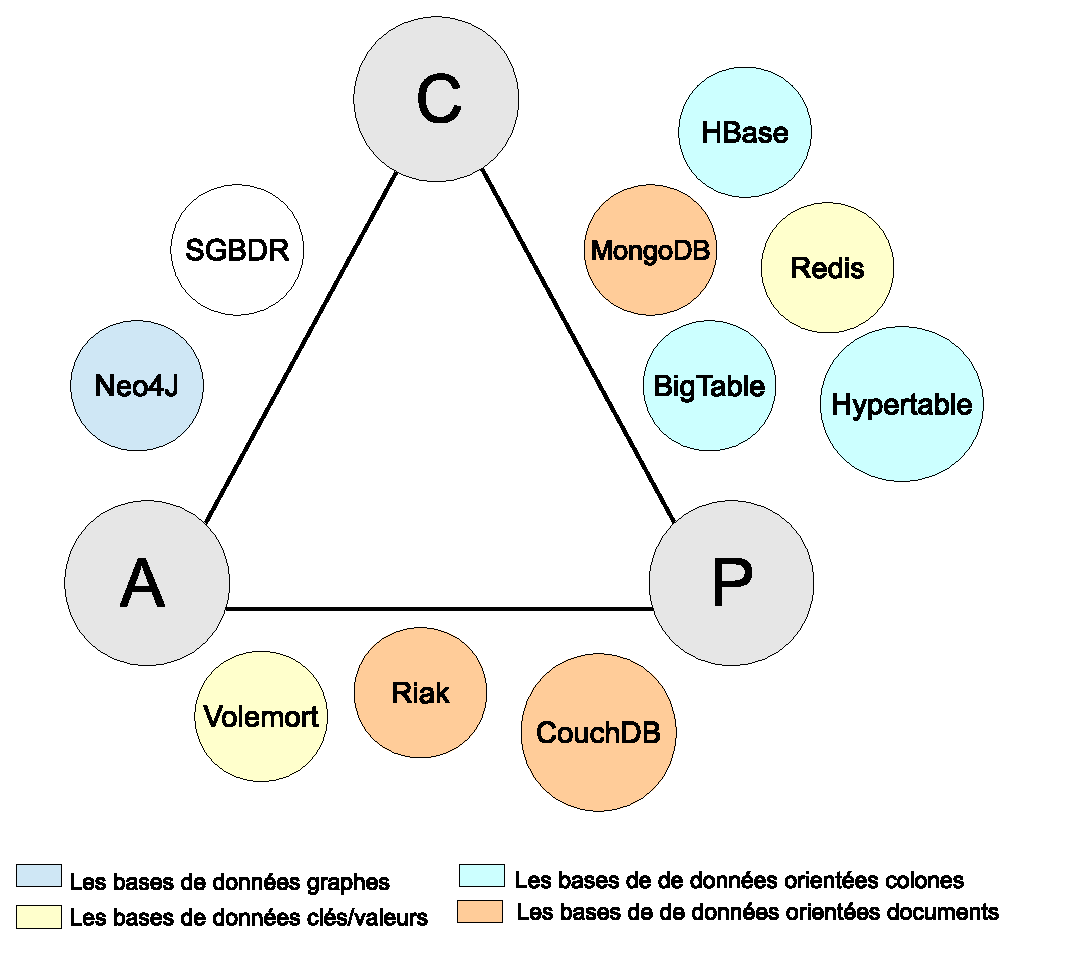
\includegraphics[width=0.96\textwidth]{figs/cap.eps}
    \caption{Le théorème CAP}
    \label{fig:cap}
\end{figure}

%%% Local Variables:
%%% mode: latex
%%% TeX-master: "../main"
%%% End:


  Le théorème de \acrshort{cap} stipule qu'il est impossible d'obtenir
  ces trois propriétés en même temps dans un système distribué et
  qu'il faut donc en choisir deux parmi les trois, Les bases de
  données relationnelles implémentent les propriétés de cohérence et
  de disponibilité (système \emph{CA}). Les bases de données
  \emph{NoSQL} sont généralement des systèmes \emph{CP} (cohérent et
  résistant au partitionnement) ou \emph{AP} (disponible et résistant
  au partitionnement), la figure \ref{fig:cap} présente le
  positionnement de quelque systèmes \emph{NoSQL} par rapport au
  théorème \acrshort{cap} .

\section{Bases de données orientées graphes}
\label{sec:graph-database-overview}
% TODO: rewrite the intro
\begin{text}
  Un grand nombre de problèmes pratiques dans différentes disciplines
  peuvent être intuitivement représentés sous forme de graphes : des
  nœuds reliés par des arcs (étiqueté ou non).

  Depuis plusieurs décennies, les développeurs ont essayé de stoker
  des ensembles de données connectés, semi-structurées à l'intérieur
  des bases de données relationnelles. Mais alors que les bases de
  données relationnelles ont été initialement conçues pour codifier
  des structures tabulaires. Cependant, les données fortement
  connectées sont traitées de manière très pauvre par les bases de
  données relationnelles. Chaque opération sur une relation dans un
  graphes ou réseau résulte en une opération de jointure dans le
  \acrshort{SGBDR}, implémentée comme une opération ensembliste entre
  l'ensemble des clés primaires de deux tables - une opération lente
  et sans capacité à monter en charge alors que le nombre de t-uples
  de ces tables augmente \cite{robinson2013graph}.

  Les bases de données orientées graphes sont donc conçues pour
  modéliser des réseaux de données fortement connectées et y naviguer
  facilement en bénéficiant de performances extrêmement élevées – un
  atout qui explique leur succès auprès de
  Facebook\footnote{\url{http://www.facebook.com}},
  LinkedIn\footnote{\url{http://www.linkedin.com}} et autres réseaux
  sociaux. Ces derniers sont devenus ces dernières années l'un de cas
  d'utilisation les plus visibles des bases de données graphes.
  LinkedIn parvient ainsi facilement à afficher le degré de séparation
  entre chaque contact, qui n'est finalement que la distance entre les
  nœuds dans le graphes représentant les personnes et leurs relations.
\end{text}

% TODO: relational vs graph database
  \subsection{Techniques de persistance des bases de données graphes}
  \label{sec:persistence-tech}
  % TODO: rewrite
  Généralement, nous pouvons distinguer trois techniques majeures du
  stockage adoptés par les systèmes de gestion des bases de données
  graphes: les bases de données graphes qui utilisent des
  \acrshort{SGBDR} comme un \emph{backend}, celles qui utilisent des
  systèmes \acrshort{nosql}, et enfin, nous avons les bases de données
  graphes natives qui fournissent ses propres implémentations du
  stockage en termes des nœuds et des arcs directement.

    \subsubsection{Bases de données graphes au-dessus de d'un stockage  SQL}
    \label{sec:graphdb-over-sql}
    % TODO: rewrite this paragraph
    Une base de donnée graphe peut être stockée dans une base de
    données relationnelle. Les étiquettes et les attributs de nœuds et
    arcs peuvent être gérés séparément dans d'autres tables et renvoyé
    par des clés étrangères. l'utilisation des \acrshort{SGBDR} comme
    un moteur de stockage a quelques avantages : des systèmes
    d'indexation évolués, un support des transactions sophistiqué, et
    le langage de requêtes \emph{SQL} qui est un standard bien établi
    avec a cycle d'apprentissage rapide.

      \begin{figure}[h]
    \centering
    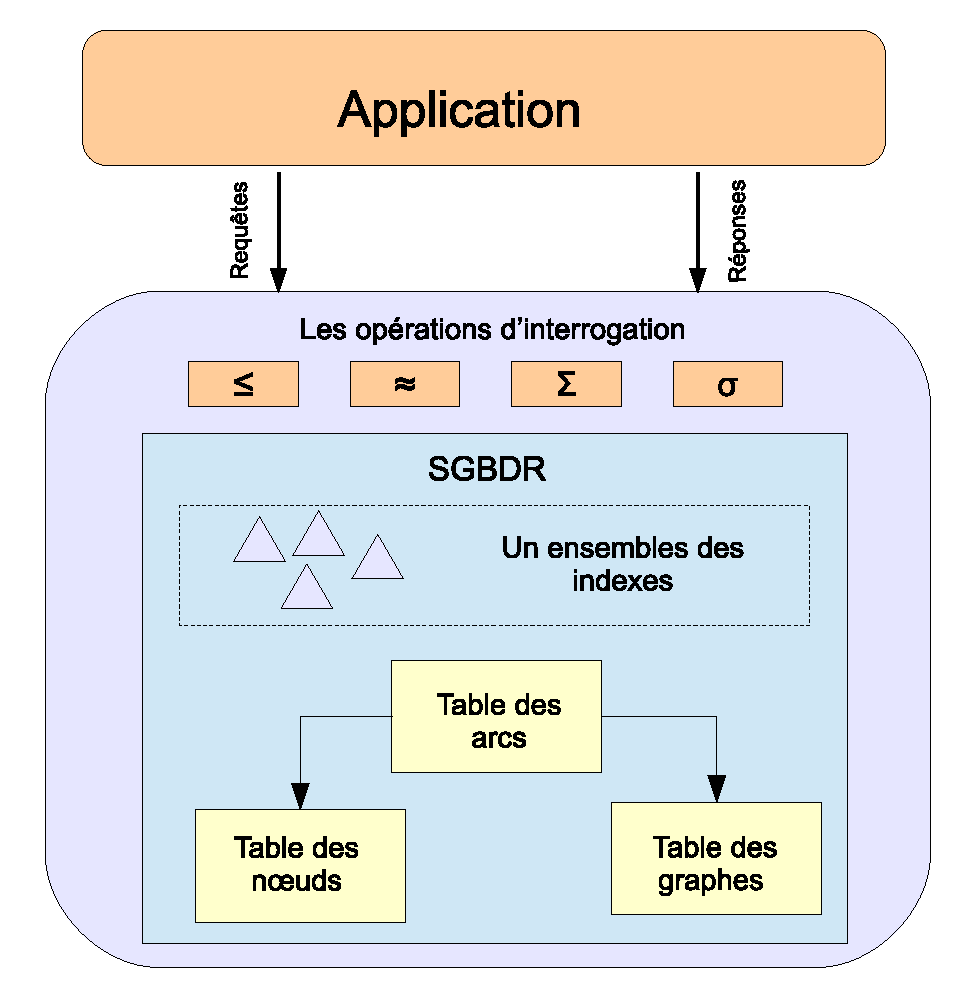
\includegraphics[width=0.8\textwidth]{figs/periscope-gq.eps}
    \caption{L'architecture du système Periscope/GQ \cite{tian2008periscope}}
    \label{fig:periscope-gq}
\end{figure}

%%% Local Variables:
%%% mode: latex
%%% TeX-master: "../main"
%%% End:


    Cette classe comprend \emph{GRIPP} \cite{trissl2007fast}, et
    Periscope/GQ \cite{tian2008periscope} développé par l'université
    de Michigan qui implémente un système de gestion des bases de
    données graphes comme une application au-dessus d'un moteur de
    stockage relationnel \emph{PostgreSQL} (ce qui est démontré dans
    la figure \ref{fig:periscope-gq}).

    % TODO: why not graphdb over SGBDR?

    \subsubsection{Bases de données graphes au-dessus d'un stackages NoSQL}
    \label{sec:graphdb-over-nosql}
    Plusieurs systèmes de base de données graphes emploient des
    systèmes \acrshort{nosql} comme un moteur de stockage interne
    offrant une meilleure scalabilité et un support fiable pour le
    partitionnement des données.

    \begin{itemize}
    \item [HypergraphDB]: \emph{HypergraphDB} \cite{hypergraphdb,
        iordanov2010hypergraphdb} est une base de donnée qui
      implémente le modèle de données \emph{``hypergraph''} où la
      notion d'un arc est étendue pour pouvoir connecter plus de deux
      nœuds, ce qui est particulièrement utile pour la modélisation
      des données tels que la représentation des connaissances,
      l'intelligence artificielle et la
      bio-informatique. \emph{HypergraphDB} utilise le modèle
      \textit{clé/valeur} de \emph{BerkeleyDB} \cite{berkeleydb} pour
      stocker toutes les informations relatives du graphe sous forme
      de pairs \textit{clé/valeur}, chaque objet du graphe (nœud ou
      arc) est identifié par un clé unique (appelé atome). Chaque
      atome est lié à un ensemble des atomes par une relation de type
      \emph{0:N} (zéro ou plusieurs atomes), ces relations forment
      également la structure typologique ``hypergraph''.

    \item [OrientDB]: \emph{OrientDB} \cite{orientdb} est un système
      de gestion de base de données graphes hybride qui combine les
      fonctionnalités d'une base orientée documents et une base
      orientée graphes avec une capacité de stockage des données
      structurées ou semi-structurées (\emph{schema-less}). il
      supporte aussi la répartition de charge à travers plusieurs
      machines et la réplication multi-maîtres tout en assurant les
      propriétés \acrshort{acid} de données. Pour les requêtes
      simples, \emph{OrientDB} s'appuie sur \emph{SQL} et utilise des
      langages de parcours des graphes comme \emph{Gremlin} afin
      d'éviter les jointures \emph{SQL} coûteuses pour les requêtes
      complexes.

      \newpage
    \item [Titan]: \emph{Titan} \cite{titan} est une base de données
      orientée graphes évolutive (\emph{scalable}) et
      transactionnelle, optimisée pour le stockage et l'interrogation
      des données graphes contenant des centaines de milliards de
      sommets et d'arcs à travers un \emph{cluster} multi-machine avec
      des schémas complexes du parcours et requêtage et une éxecution
      en temps réal. \emph{Titan} utilise une multitude des systèmes
      \emph{NoSQL} comme un moteur de stockage (\emph{backend}), par
      exemple, \emph{Hbase}, \emph{Cassandra}, \emph{BerkeleyDB},
      cette diversité offre une flexibilité en terme des
      caractéristiques \emph{CAP} \ref{sec:cap} assurées par le
      système.
    \end{itemize}

    \subsubsection{Les bases de données graphes natives}
    \label{sec:graphdb-native}
    Les bases de données graphes natives possèdent leurs propres
    systèmes de fichiers pour stocker les données au lieu de compter
    sur des moteurs de stockage tiers. Ces bases de données sont
    optimisés pour stocker et gérer les données \textbf{fortement}
    connectées où la performance et la disponibilité sont
    primordiales.

    \begin{itemize}
      %TODO: translate + enhance
    \item [Neo4j]: Neo4j \cite{neo4j} is a disk-based transactional
      graph database that implemented in Java. It is one the most
      popular graph databases. Besides the advantages in traversing
      the graph data like other graph databases, it highlights its
      full ACID transaction support and convenient REST server
      interfaces. Those features ensure it to be suitable for its
      enterprise solutions. It also pro- vides its own query language
      called Cypher, which can handle different kinds of queries with
      syntax. At the same time, their developers make APIs for almost
      all of program- ming languages to access their graph database.

      %TODO: enhance Allegrograph paragraph
    \item [AllegroGraph]:\emph{AllegroGraph} \cite{allegrograph} est
      un système performant de persistence des données graphes avec un
      stockage natif, implémenté initialement comme une base de
      \acrshort{rdf}, avec un support d'interrogation
      \acrshort{sparql} et un service \acrshort{rest}
      \cite{fielding2000architectural}. Similaire à \emph{Neo4j},
      \emph{Allegrograph} garantis la satisfaction des propriétés
      \acrshort{acid} d'atomicité, cohérence, isolation et
      durabilité. \emph{AllegroGraph} supporte \acrshort{sparql},
      RDFS++ et Prolog pour des applications clientes multiples.

    \item [Sparksee]: \emph{Sparsity} \cite{sparksee} (auparavant
      connu sous le nom \emph{DEX}) est un système natif de stockage
      de données graphes persistants et temporaires. \emph{Sparsity}
      focalise sur la gestion et l'interrogation des géantes bases de
      données graphes à haute performance. En encodant les matrices
      d'adjacences en \emph{bitmap}, le système a une gestion d'espace
      disque compact et efficace afin de d'assurer une trés bonne
      performance.

    \item [InfiniteGraph]: \emph{InfiniteGraph} \cite{infinitegraph}
      est un système distribué de gestion des bases de données graphes
      qui supporte des grandes masses évolutives de données
      (\emph{large-scale}) avec une capacité d'analyse efficace des
      graphes et une bonne prise en charge des algoritmes distribués
      du parcours. \emph{InfiniteGraph} fournis une variété
      d'implémentations pour des différents systèmes (serveurs
      d'application, les plateformes de \emph{cloud computing} et les
      systèmes embarqués).

    \item [FlockDB]: FlockDB \cite{flockdb} is an open source
      distributed, fault-tolerant graph database for managing wide but
      shallow network graphs. It was initially used by Twitter to
      store relationships between users, e.g. followings and
      favorites. FlockDB differs from other graph databases,
      e.g. Neo4j in that it is not designed for multi-hop graph
      traversal but rather for rapid set operations, not unlike the
      primary use-case for Redis sets. Since it is still in the
      process of being packaged for outside of Twitter use, the code
      is still very rough and hence there is no stable release
      available yet. FlockDB was posted on GitHub shortly after
      Twitter released its Gizzard framework, which it uses to query
      the FlockDB distributed datastore.
    \end{itemize}

    \begin{figure}[!hr]
    \centering
    \begin{subfigure}[h]{0.7\textwidth}
        \centering
        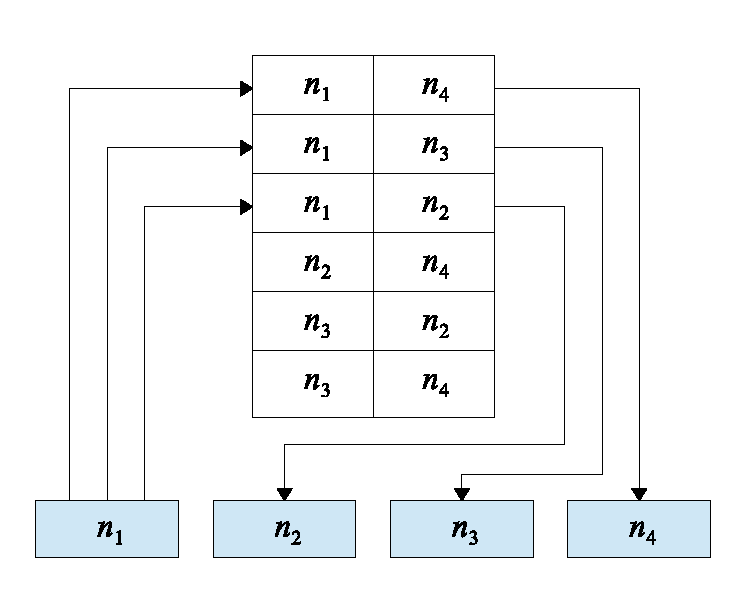
\includegraphics[width=\textwidth]{figs/global-graph-index-table.eps}
        \label{fig:global-graph-index-table}
    \end{subfigure}

    \begin{subfigure}[h]{0.45\textwidth}
        \centering
        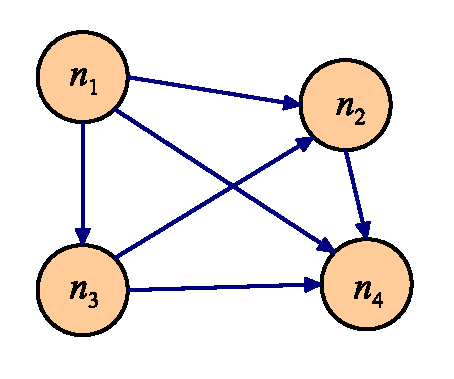
\includegraphics[width=\textwidth]{figs/global-graph-index.eps}
        \label{fig:global-graph-index}
    \end{subfigure}

    \caption{Une indexation global des données fortement connectées}
    \label{fig:gpi}
\end{figure}

%%% Local Variables:
%%% mode: latex
%%% TeX-master: "../main"
%%% End:


  \subsection{Détails d'implémentation}
  \label{sec:graph-internals} 
  \begin{itemize}

  \item [Index-free adjacency]:Index-free adjacency (Neo4j) makes the
    nodes contain direct reference/index to their adjacent neighboring
    nodes. This means it is unnecessary to maintain a global index for
    relationships between nodes/edges. This term has similar concept
    as adjacency list, except the local indices for each node may also
    contain the property of nodes and edges.  By using Index-free
    adjacency, time of queries based on traversal the graph will be
    inde- pendent of the total size of the graph.


  \item [Vertex Centric Indices]: Vertex Centric Indices (Titan) is
    used to find if a certain node is connected to another node by
    their unique identifier. As the desciption in the second chapter,
    most networks in real world can be fit with power-law
    distribution. It means most of the nodes do not have large amount
    of neighbors. But there do exist some supernodes which connect
    large number of nodes, these supernodes result in the small world
    phenomena. For example, US president Barack Obama currently has
    38,844,920 followers on Twitter. Appling graph term to it, the
    vertex Obama is considered a supernode in Twitters network. Obama
    send a tweet, it will be sent to more than 38 million accounts on
    Twitter. To store these supernodes, graph database like Titan will
    first build an index to classify the edges according to edges
    label or property, because there may not be just one type of edge
    for the supernode. Then it sorts the incident nodes of the
    supernode. By doing these, when querying a vertexs neighbor,
    linear scans of incident edge (O(n)) can be reduced to at least
    O(log(n)).

  \item [Bitmaps representation of graphs]: Graph database like DEX
    uses adjacency matrix to multiple small indices to improve the
    management performance. The indices will be encoded into
    bitmaps. The first bit represent the first node insert to the
    graph, the last bit represent the latest coming node.  The
    relationship between each bit and node will be kept in an index,
    when there is a new node inserted, the index will be updated. To
    add an edge between two nodes, it just needs to update the related
    bit to 1. DEX also uses key-value maps to provide the index of
    full data access to complement the bitmaps. Because the adjacency
    is usually sparse, the compressed bitmaps will use the space more
    efficiently. Another advantage is that the insert, delete
    operations are all bit operations, which are much faster than
    common operation for objects.


  \item [Write Ahead Log]: Different from other techniques discussed
    in this section, Write Ahead Log (WAL) is a technique that widely
    used in transactional database. In transactional systems,
    atomicity and durability (from the ACID guarantees) are provided
    by using a WAL. All modifications during a transactional are
    persisted on disk as they are requested but are not actually
    stored. After the transactional is committed, only then the
    modifications of transactions will be really stored on the
    database and the transactional is removed from is temporary
    place. In Neo4j, WAL stores 3 files, a marker file, keeping track
    of which of the other two is the current active log file
    [23]. When the transaction finished normally, marker file will be
    marked as healthy and two other log files are removed. But if the
    process crashes, the marker file will be indicated as not
    finished, it will go look at the last active log. If the log has
    all of information of the transaction, it will do recovery by
    creating a new transaction. Otherwise it will do rollback, which
    means remove the transaction files in temporary space. This
    technique has ensured the atomicity of the transaction process. In
    most of graph databases API, we can call commit () to finish the
    transaction.
  \end{itemize}
  \newpage
  \subsection{Comparaison}
  \label{sec:graphdb-comp}
  % \begin{table}[htb!]
  \centering
  \begin{tabular}{|lcccc|}
  \end{tabular}
  \newline
  \caption{Comparaison des bases de données graphes}
  \label{tab:graphdb-comp}
\end{table}

%%% Local Variables:
%%% mode: latex
%%% TeX-master: "../main"
%%% End:


 \newpage
\section{Langages d'interrogation des bases de données graphes}
\label{query-languages}

Les langages de requêtes ont toujours été la clé du succès des
systèmes de gestion des bases de données. La prévalence des
\emph{\acrshort{SGBDR}} dans les dernières décennies est étroitement
couplé avec le succès du \emph{SQL}. Des divers langages ont été
définis pour exprimer des requêtes vis-à-vis plusieurs dépôts de
données, par exemple, \emph{XQuery} \cite{boag2002xquery} et
\emph{XPath} \cite{clark1999xml} pour les bases de données
\emph{\acrshort{xml}}, \emph{QQL} \cite{alashqur1989oql} pour les
bases de données orientées objets et \acrshort{sparql}
\cite{prud2008sparql} pour les triplestores (les bases de données
\emph{RDF}). Dans cette section on va présenter les langages de
requêtes les plus utilisée pour l'interrogation des bases de données
graphes.

  % TODO: make a simple graph example
  \subsection{SPARQL}
  \label{sec:sparql}

  \acrshort{sparql} \cite{prud2008sparql} est un langage populaire de
  requêtes pour les données \acrshort{rdf}, il est reconnu comme l'une
  des technologies clés du Web sémantique. Le standard
  \acrshort{sparql} est largement utilisé pour exprimer des
  interrogations à travers diverses sources de données graphes vues
  comme des triplestores \acrshort{rdf}. Il est capable de rechercher
  des motifs de graphe (\emph{graph patterns}) ainsi que leurs
  conjonctions et leurs disjonctions. Les résultats des interrogations
  \textsc{SPARQL} peuvent être des ensembles de résultats ou des
  graphes \acrshort{rdf} qui peuvent être retournés via
  \acrshort{http} dans une variété de formats tels que \acrshort{xml},
  HTML ou \acrshort{json}

  % syntaxe
  % example
  % graph-db support

  {\color{red} \textsc{SPARQL} is supported by some databases such as
    AllegroGraph natively. Other graph databases like Neo4j also
    support \textsc{SPARQL} by applying plugin Linked Data.  }



  \subsection{Gremlin}
  \label{sec:gremlin}
  \emph{Gremlin} \cite{gremlin-wiki} est un langage de domaine
  spécifique (\acrshort{DSL}) de bas niveau pour le parcours des
  graphes attribués, il trouve ses applications dans les domaines de
  la recherche, l'analyse et la manipulation des bases de données
  orientées graphes qui implémentent le modèle \emph{Blueprints}
  \cite{blueprints} de données. \emph{Gremlin} \cite{gremlin-wiki} est
  un projet open source développé et maintenu par \emph{TinkerPop}.

  Le syntaxe \emph{Gremlin} est basée sur \emph{XPath} de manière à
  être capable d'exprimer des descriptions de parcours même profonds
  avec des expressions simples et compactes.

  % example

  La distribution \emph{Gremlin} (maintenu par \emph{TinkerPop}) est
  supporté par la plupart des bases de données graphes via des
  langages \emph{JVM} comme \emph{Java}, \emph{Groovy} et
  \emph{Scala}, parmi ces \acrshort{SGBD} graphes nous trouvons
  \emph{Neo4j}, \emph{Titan} et \emph{OrientDB}.

  \subsection{Cypher}
  \label{sec:cypher}
  \emph{Cypher} \cite{cypher-docs} est un langage des requêtes
  déclaratif pour interagir avec les bases des données graphes
  \emph{Neo4j}, développé et maintenu par \emph{Neo Technology}. Il
  permet d'effectuer des requêtes et mises jour du graphe efficaces
  sans avoir écrire de traversiers (parcours) d'une manière
  procédurale.

  En étant un langage déclaratif, \emph{Cypher} se concentre sur la
  clarté d'exprimer \textit{quoi retrouver dans un graphe et non
    comment le faire}. Ceci est en contraste aux langages impératifs
  comme Java et aux langages script comme \emph{Gremlin}
  \ref{sec:gremlin}, ce qui rend le fait d'optimisation de requêtes un
  détail d'implémentation non exposé aux utilisateurs. \emph{Cypher}
  est inspiré de plusieurs approches et construit sur des pratiques
  établies pour l'interrogation expressif des bases de données. La
  plupart des mots clés comme \verb|WHERE| et \verb|ORDER BY|, et La
  concordance de patterns sont hérités directement des langages
  déclaratifs comme \emph{SQL} et \emph{SPARQL} \ref{sec:sparql} avec
  quelque propriétés inspirés des langages fonctionnels comme
  \emph{Haskell} et \emph{ML}.

  Le langage \emph{Cypher} comporte un nombre de clauses distinctes,
  des clauses pour l'interrogation du graphe comme:
  \begin{itemize}
  \item [\texttt{MATCH}]: Utilisé pour pour décrire Le pattern du graphe
    à correspondre, principalement sur la base de relations entre les
    nœuds du graphe.
  \item [\texttt{WHERE}]: Sert à un critère de filtrage.
  \item [\texttt{RETURN}]: Spécifie ce qu'il faut retourner comme
    résultat finale de requête.
  \end{itemize}

  \emph{Cypher} contient en outre des clauses pour l'écriture, la mise
  à jour et suppression de données, par exemple:

  \begin{itemize}
  \item [\texttt{CREATE}]: Crée des nœuds ou des relations.
  \item [\texttt{SET}]: Affecte des valeurs aux propriétés..
  \item [\texttt{DELETE}]: supprime des noeuds, relations ou propriétés.
  \end{itemize}

  % graph-db support

  % TODO:comparaison

  \section{Conclusion}

  % TODO: Neo4j internals
%%% Local Variables:
%%% mode: latex
%%% TeX-master: "../main"
%%% End:
